\section{Additional tool analysis}
\label{appendix:tool_analysis}

\begin{figure*}[h]
    \centering
    \begin{subfigure}[b]{0.32\textwidth}
    \centering
    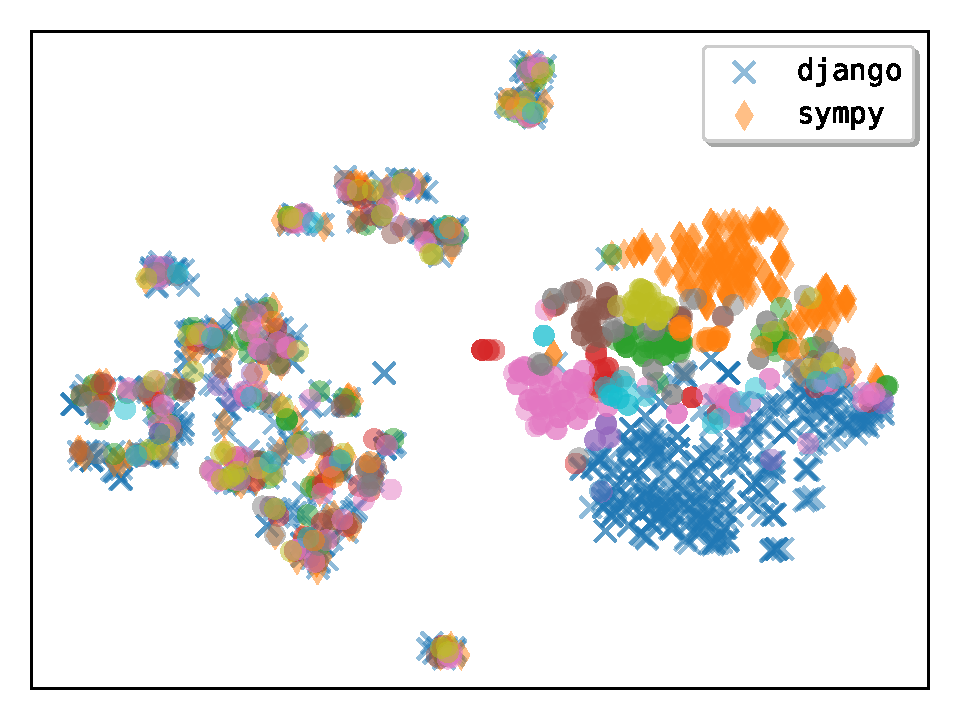
\includegraphics[width=\textwidth]{appendix/figs/tsne_verified_claude_repo.pdf}
    \caption{Tools in \swebench Verified}
    \label{fig:tool_verified_repo}
\end{subfigure}
\begin{subfigure}[b]{0.32\textwidth}
    \centering
    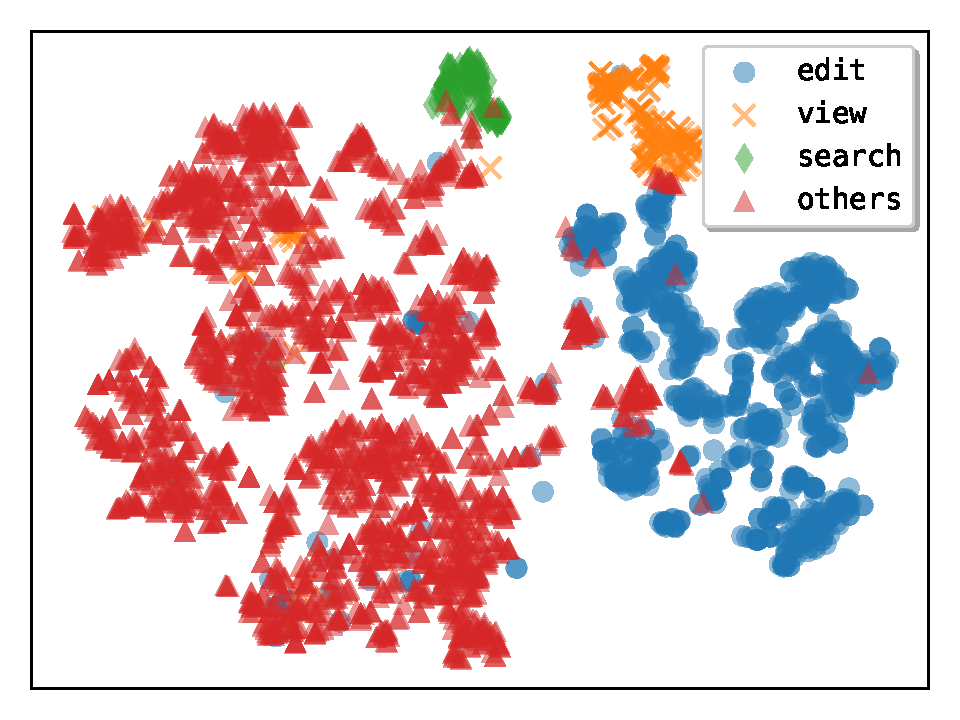
\includegraphics[width=\textwidth]{appendix/figs/tsne_pro_claude_tool_use.pdf}
    \caption{Tools in \swebenchpro{}}
    \label{fig:tool_pro_tool_name}
\end{subfigure}
\caption{
Additional 2 dimensional t-SNE visualization of tools generated by \claudesonnetfourfive{} on \swebench Verified and \swebenchpro.
We label and display the embedding based on the repository name (Figure~\ref{fig:tool_verified_repo}) and tool name (Figure~\ref{fig:tool_pro_tool_name}).
Note that for Figure~\ref{fig:tool_verified_repo}, we only label two repositories in the legend due to space considerations. 
The two repositories were chosen as they have representative distinct clusters.
}
\end{figure*}

We perform additional tool analysis similar to the ones done in Section~\ref{sec:tool_analysis}.
We added the missing results including the visualization based on repository used for \swebench Verified and tool name for \swebenchpro.
Note that we did not include any results based on programming language for \swebench Verified since they are all repositories in Python.
We observe similar patterns to the main evaluation.

To perform this analysis, we use \CodeIn{sklearn} implementation of PCA with \CodeIn{n\_components} of 50. 
We then use the t-SNE implementation from \CodeIn{sklearn} with \CodeIn{max\_iter} of 1000.
